\chapter{Normal Sampling}

\begin{tcolorbox}[title=]
    It’s nice to know that standard normal random variables exist and are well
    behaved, but can we sample from a standard normal distribution?

    Let’s be clear on what we want to do. We would like to find an algorithm
    $\mathcal{A}$ that takes some uniformly random numbers in $[0, 1]$, and
    generates an output $x \in \mathbb{R}$. The algorithm should use randomness
    of the numbers it receives in such a way that the output $x$ of the algorithm
    is distributed standard normally. Denote by $f_\mathcal{A}(x)$ the PDF of the
    algorithm’s output - a random variable - $X$. We wish that for every $x \in
    \mathbb{R}$,

    \begin{equation*}
        f_\mathcal{A}(x) = \dfrac{1}{\sqrt{2\pi}}e^{\sfrac{-x^2}{2}}
    \end{equation*}

    We will show and then use a general theorem to find such an algorithm. A
    note on notation: we shall use $f_X$ to denote the PDF of the random variable
    $X$ and $F_X$ to denote the CDF.
\end{tcolorbox}

\section*{\colS{$\S$} Task A \hfill \normalfont \large [2]}

\begin{tcolorbox}
    Prove the theorem below.

    \vspace{10pt}
    \begin{mdframed}[backgroundcolor=lightyellow, linecolor=darkyellow,
    linewidth=1.5pt]
        \textbf{Theorem 3.}
        \textit{Let $X$ be a continuous real-valued random variable with CDF $F_X:
         \mathbb{R} \xrightarrow{} [0, 1]$. Assume that $F_X$ is invertible. Then
         the random variable $Y := F_X(X) \in [0, 1]$ is uniformly distributed in
         $[0, 1]$.}
    \end{mdframed}
\end{tcolorbox}

% Solution A

We are given the random variable $Y$, where $Y:= F_X(X)$, where $X$ is a
continuous random variable with its CDF as $F_X: \mathbb{R} \xrightarrow{}
[0, 1]$.

We proceed by finding the CDF $F_Y$ of $Y$.

\begin{equation}
    \begin{aligned}
        F_Y(Y)
        &= \text{P}(Y \le y) \\
        &= \text{P}(F_X(X) \le y).
    \end{aligned}
    \label{e2.1}
\end{equation}

As we know, $F_X$ is a continuous, monotonically increasing, and invertible
function; we get

\begin{equation}
    \begin{aligned}
        F_X(X) \le y \implies X \le F_X^{-1}(y)
    \end{aligned}
    \label{e2.2}
\end{equation}

From \ref{e2.1} and \ref{e2.2}, we have

\begin{equation}
    \begin{aligned}
        F_Y(Y) = \text{P}(X \le F_X^{-1}(y))
    \end{aligned}
    \label{e2.3}
\end{equation}

Now, by the definition of $F_X$, we can rewrite the RHS of \ref{e2.3} as

\begin{equation}
    \begin{aligned}
        F_Y(Y) &= \text{P}(X \le F_X^{-1}(y)) \\ 
        &= F_X(F_X^{-1}(y)) = y \\
        &= y \\
        \implies F_Y(Y) &= y.
    \end{aligned}
    \label{e2.4}
\end{equation}

Since $F_Y(y) = y$, the CDF of $Y$ is that of a uniform random variable on
$[0, 1]$. Therefore, $Y$ is uniformly distributed on $[0, 1]$.

\section*{\colS{$\S$} Task B \hfill \normalfont \large [2]}

\begin{tcolorbox}
    Suppose we are given a random variable $Y$, uniform over $[0, 1]$. Explain
    how an algorithm $\mathcal{A}$ may be constructed taking as input a sample
    $y$ according to the distribution of $Y$ (so the algorithm is given just one
    uniformly random number in $[0,1]$), such that for every $u \in \mathbb{R}$,
    we have

    \begin{equation*}
        F_\mathcal{A}(u) = F_X(u).
    \end{equation*}
    
    In other words, the output of $\mathcal{A}$ has the same cumulative
    distribution function as $X$, and upon taking the derivative, it has the same
    PDF.
\end{tcolorbox}

% Solution B

\noindent \hypertarget{3bNote}{\textbf{Note:}} We are assuming that $F_X$ is
invertible (and obviously monotonic).
\vspace{10pt}

To construct an algorithm $\mathcal{A}$ that transforms a uniformly random
variable $Y$ over $[0, 1]$ into a random variable with the same cumulative
distribution function (CDF) as $X$, we can use the \textbf{Inverse Transform
Sampling} method. (The most common method used for this purpose; this is the one
which I learnt in my SoC.)

\subsection*{The Algorithm $\mathcal{A}$:}

\begin{enumerate}
    \item \textbf{Compute the Inverse CDF:}
        Let $F_X(u)$ be the CDF of the target random variable $X$. Find the
        inverse of this CDF, denoted as $F_X^{-1}(u)$.
    \item \textbf{Generate a Uniform Random Variable:}
        The input to the algorithm $\mathcal{A}$ is a sample $y$ drawn from the
        uniform distribution over $[0, 1]$.
    \item \textbf{Transform Using the Inverse CDF:}
        Set the output of the algorithm as
        \begin{equation}
            \begin{aligned}
                \mathcal{A}(Y) = F_X^{-1}(Y) \\
                F_{\mathcal{A}}(u) = \text{P}(\mathcal{A}(Y) \leq u) \\
            \end{aligned}
            \label{e2.5}
        \end{equation}
\end{enumerate}

\subsection*{Verifying that $\mathcal{A}$ works:}

We need to show that $F_\mathcal{A}(u) = F_X(u)$ for all $u \in \mathbb{R}$. Using
\ref{e2.5} and the \hyperlink{3bNote}{note}:

\begin{equation*}
    \begin{aligned}
        F_\mathcal{A}(u) &= \text{P}(\mathcal{A}(Y) \leq u) \\
        &= \text{P}(F_X^{-1}(Y) \leq u) \\
        &= \text{P}(Y \leq F_X(u)) \\
        &= F_Y(F_X(u)) = F_X(u)
    \end{aligned}
\end{equation*}
where $F_Y$ is the CDF of the uniform distribution, and since $Y$ is uniformly
distributed over $[0,1]$, $F_Y(y) = y$.

\section*{\colS{$\S$} Task C \hfill \normalfont \large [8]}

\begin{tcolorbox}
    In this task, you will use the \texttt{numpy.random} module to generate random
    numbers uniformly in $[0, 1]$ and the \texttt{norm} class (gives you access to
    $F_X$ and $F_X^{-1}$ for a Gaussian random variable $X$) from
    \texttt{scipy.stats} to sample from a Gaussian. In particular,

    \vspace{10pt}
    \begin{itemize}
        \item Write a Python function \texttt{sample(loc, scale)} that samples
        from the Gaussian with mean at $x$ = \texttt{loc} and standard deviation
        \texttt{scale}.
        \item Generate $N = 1e5$ independent samples using the function above for
        the four-parameter choices $(\mu, \sigma^2) = (0, 0.2), (0, 1.0), (0,
        5.0), (-2, 0.5)$.
        \item Plot the samples for each parameter choice using
        \texttt{matplotlib.pyplot}. You should roughly reproduce the shape of the
        plot of the four Gaussians from the lecture slides (i.e., figure
        \ref{fig_q2ca}). The figure \ref{fig_q2cb} is a plot of the samples; it
        mimics the top plot of the different PDFs, confirming that we have indeed
        sampled from the different Gaussian PDFs. Save the plot in
        \texttt{2c.png}.
    \end{itemize}

    \begin{figure}[H]
        \centering
        \begin{subfigure}[l]{0.5\textwidth}
            \centering
            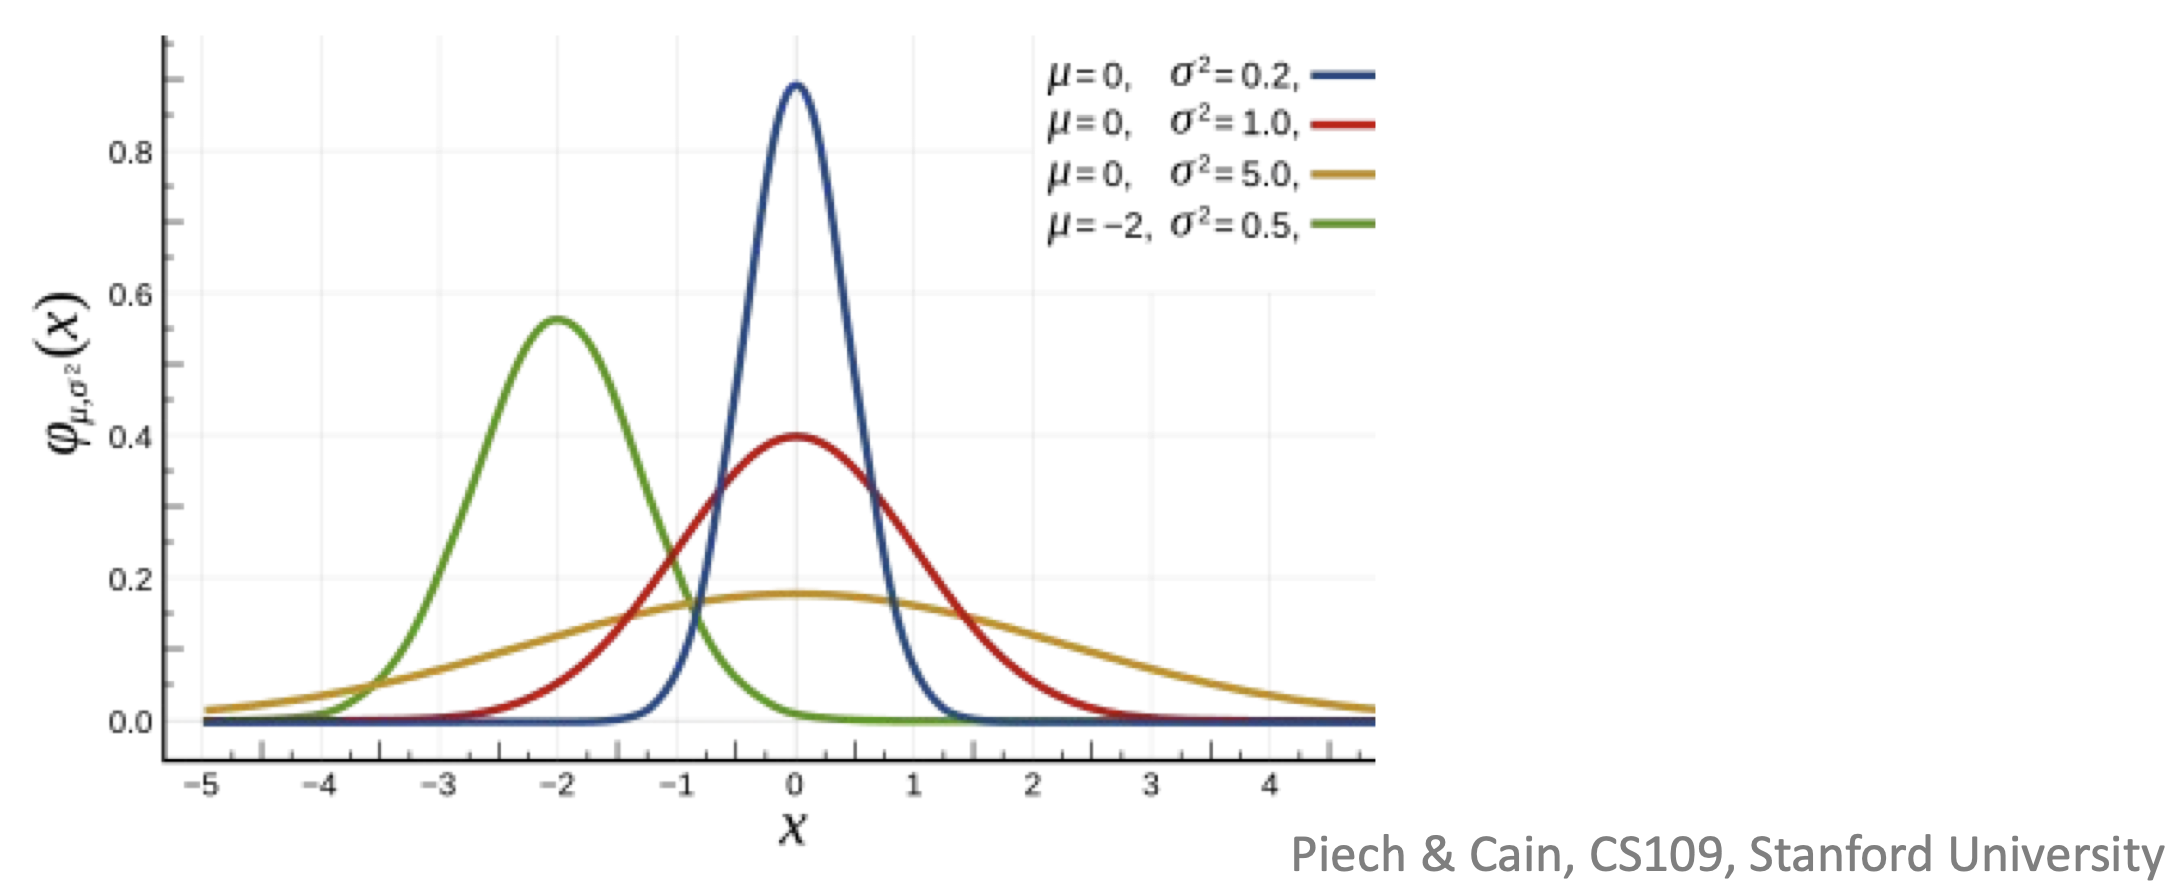
\includegraphics[width=\textwidth]{assets/images/q2c1.png}
            \caption{Gaussian}
            \label{fig_q2ca}
        \end{subfigure}
        \begin{subfigure}[r]{0.4\textwidth}
            \centering
            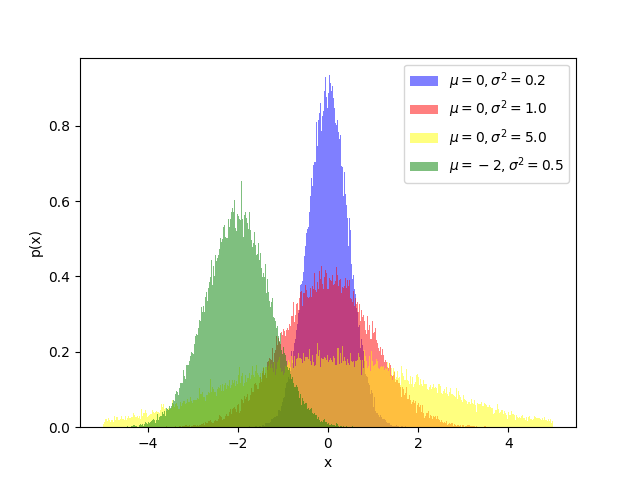
\includegraphics[width=\textwidth]{assets/images/q2c2.png}
            \caption{The figure to be reproduced}
            \label{fig_q2cb}
        \end{subfigure}
        \caption{The Bell curve, from uniformly random numbers.}
    \end{figure}
    
    You may not use the builtin \texttt{numpy.random.normal} or
    \texttt{random.randn} functions that directly sample from Gaussians for this
    task.
    
    For the plot of the samples, you may not use kernel-density estimation
    (\texttt{kde}) tools; \texttt{matplotlib.pyplot} by itself is sufficient.
    
    (You can use these if you wish for the next problem, however). Please write
    all your code for this task in one file called \texttt{2c.py}.
\end{tcolorbox}

% Solution C

For the the function \texttt{sample}, we use the result \ref{e2.5} derived in
Task B. We use the \texttt{norm} class from \texttt{scipy.stats} library. The
strategy is to use the PPF (Inverse CDF) function of the \texttt{norm} class and
pass the uniform randoms generated from \texttt{np.random.random} to it, to
generate the \textbf{Gaussian RV}. The code for the function is at
code:\ref{code:2.1}.

\begin{lstlisting}[caption={The function \texttt{sample}}, label={code:2.1}]
import numpy as np
from scipy.stats import norm


def sample(loc: float, scale: float, size: int = 100000) -> np.ndarray:
    """
    Samples from a Gaussian using `scipy.stats.norm` and `np.random`
    """

    uniform_randoms = np.random.random(size)

    # PPF - Percent Point Function - Inverse of the CDF
    gaussian_randoms = norm.ppf(uniform_randoms, loc=loc, scale=scale)
    return np.array(gaussian_randoms)
\end{lstlisting}

Some of the reproduced images are \ref{fig_a2c1} and \ref{fig_a2c2}:

\begin{figure}[H]
    \centering
    \begin{subfigure}{0.8\textwidth}
        \centering
        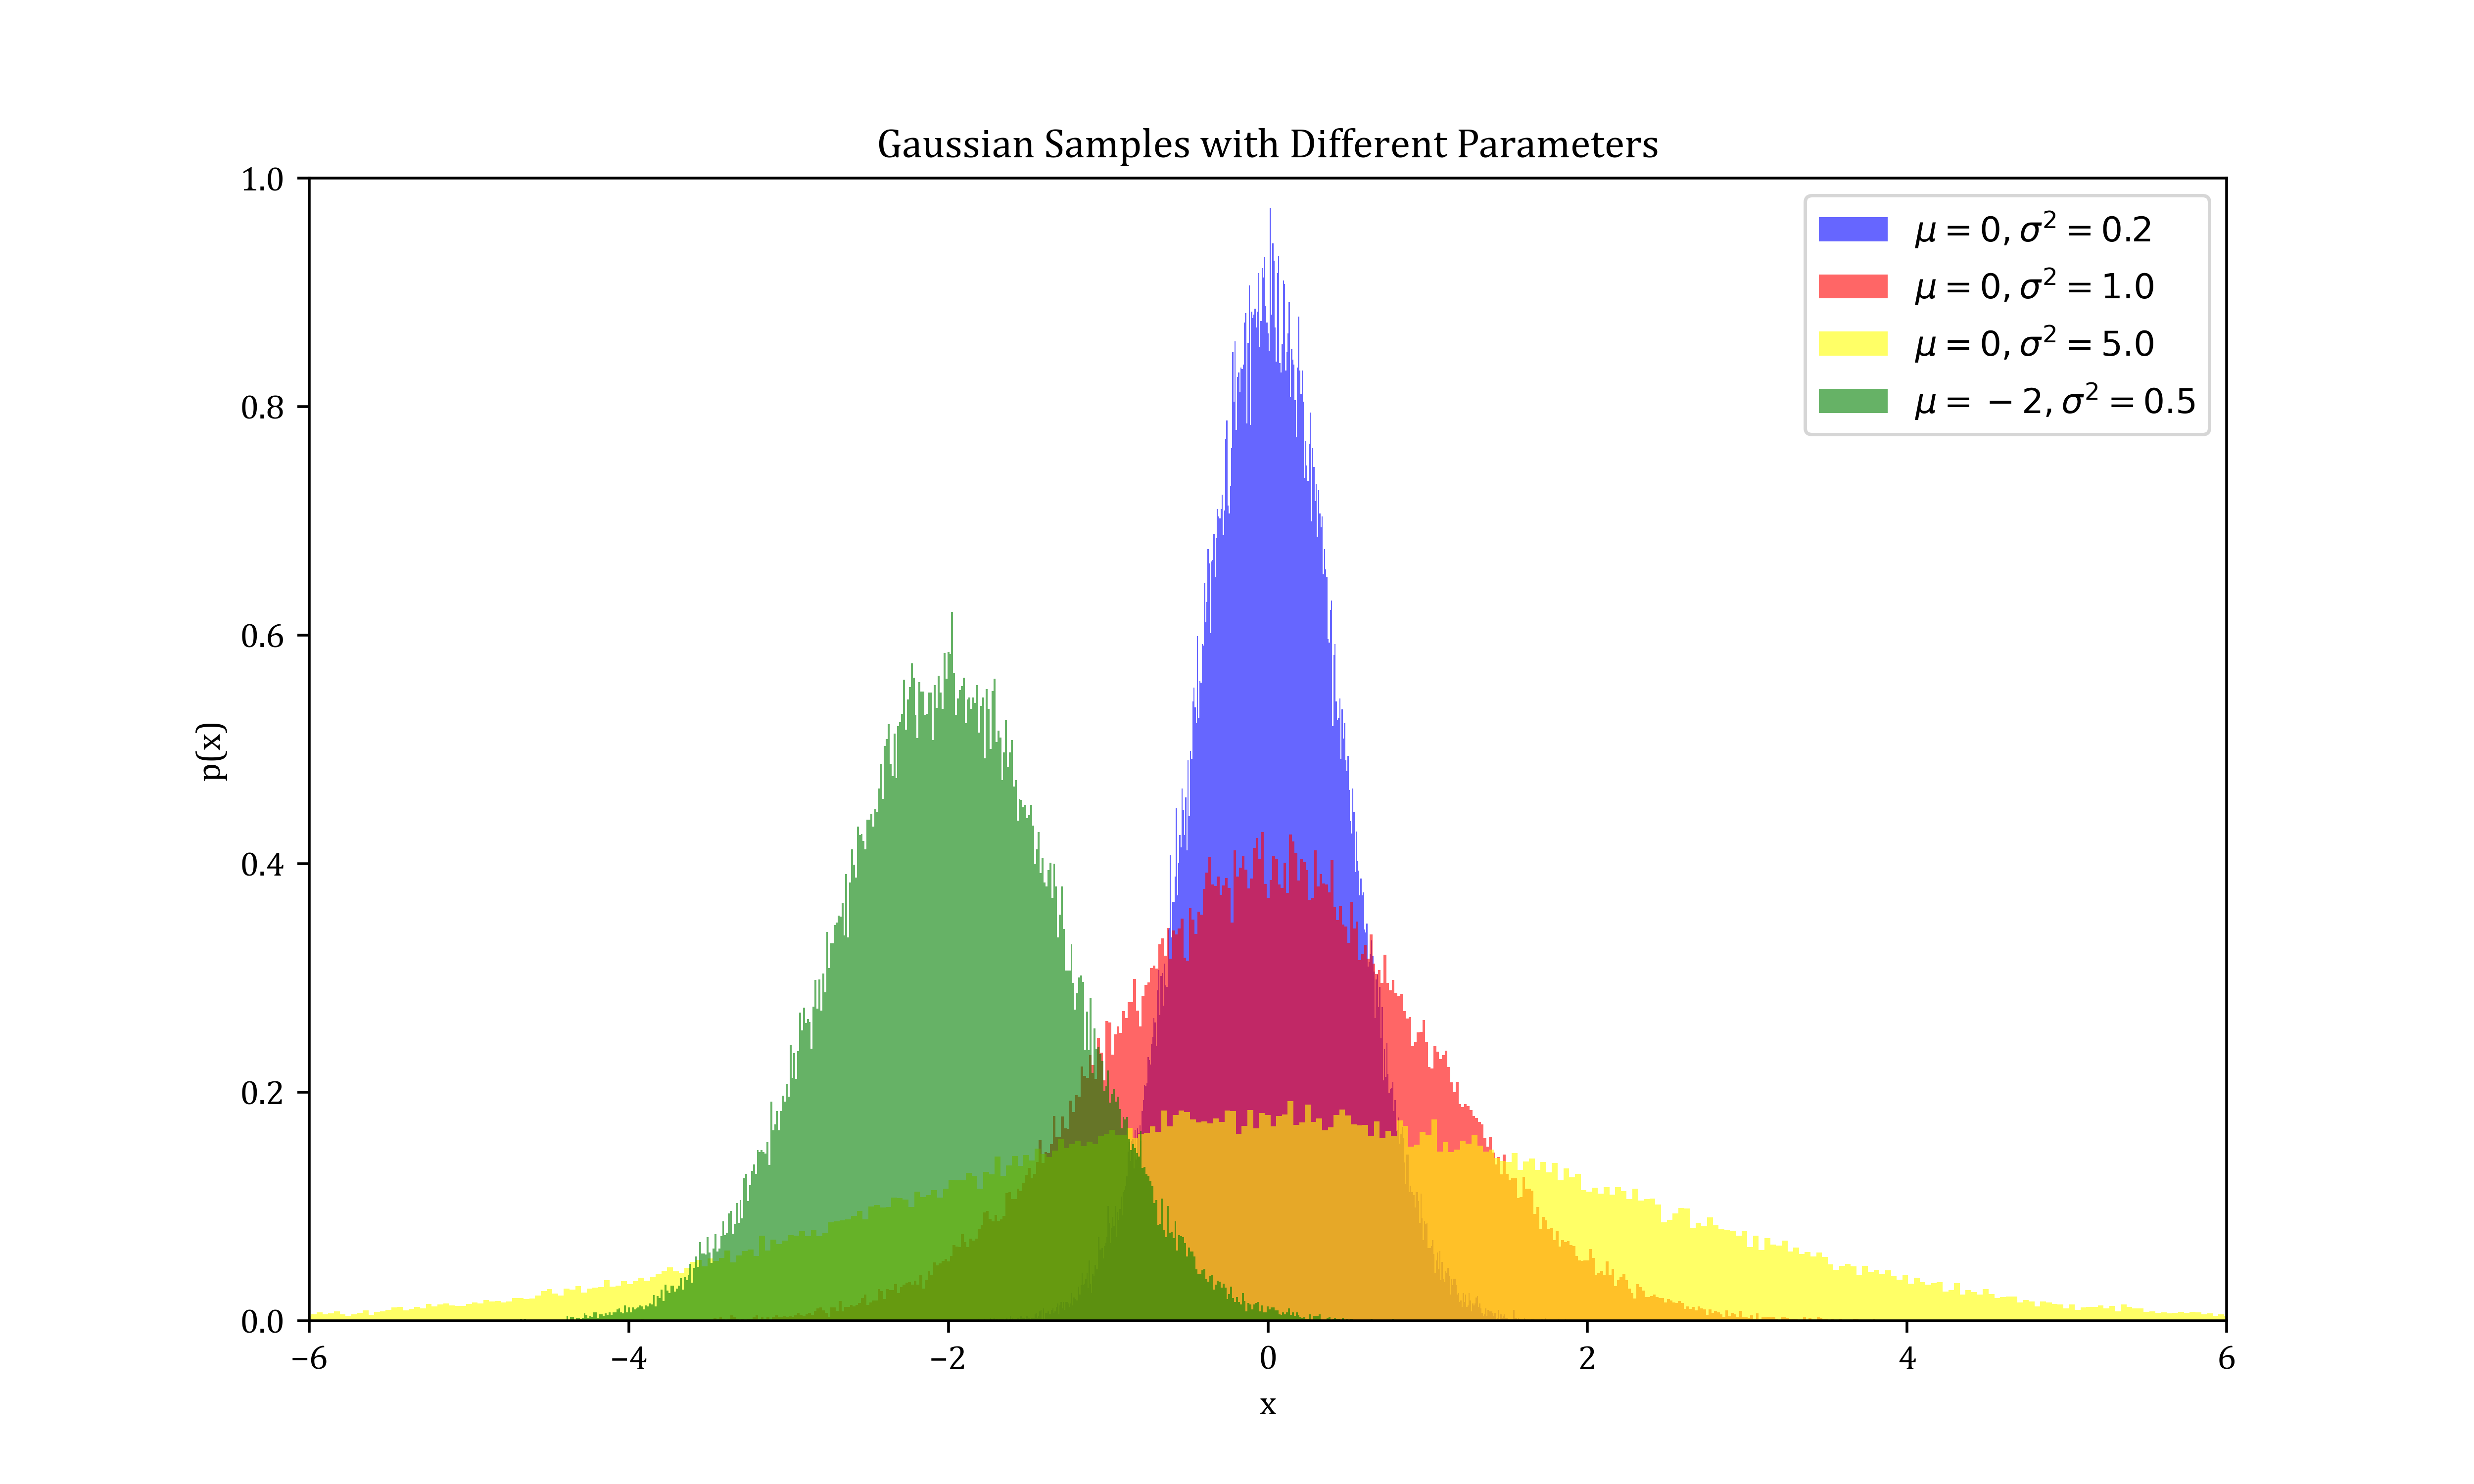
\includegraphics[width=\textwidth]{assets/images/a2c1.png}
        \caption{}
        \label{fig_a2c1}
    \end{subfigure}
    \begin{subfigure}{0.8\textwidth}
        \centering
        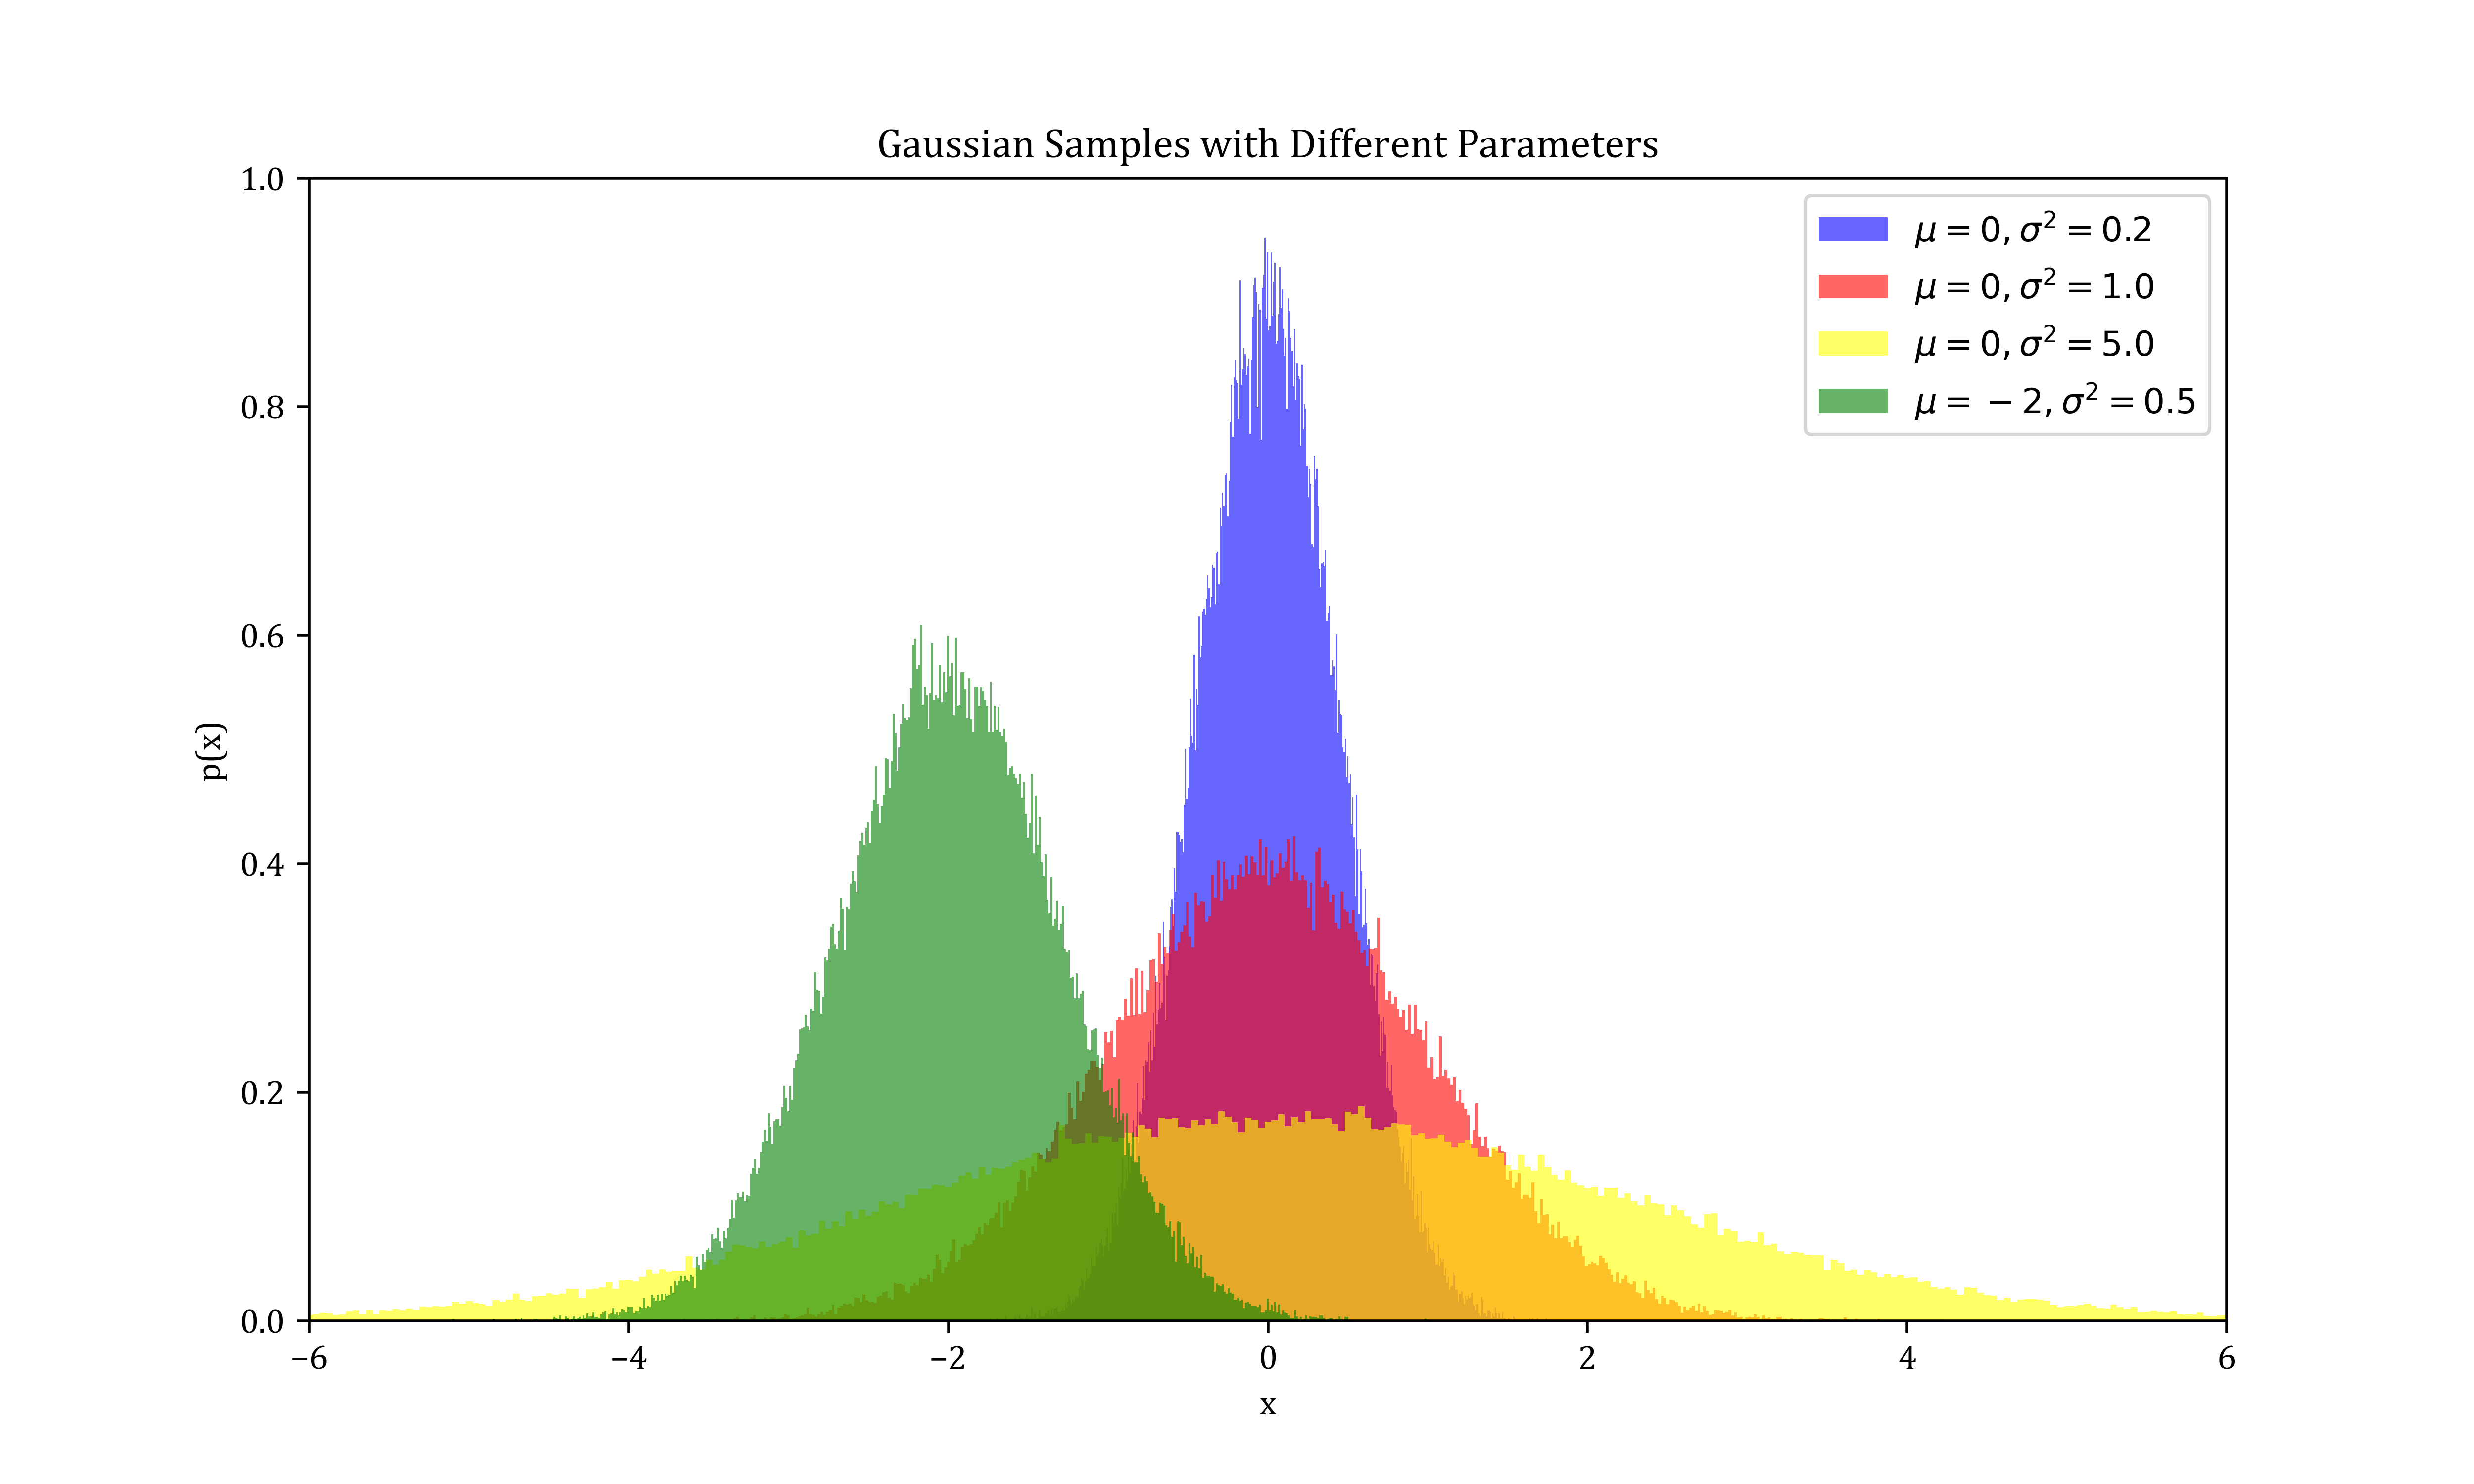
\includegraphics[width=\textwidth]{assets/images/a2c2.png}
        \caption{}
        \label{fig_a2c2}
    \end{subfigure}
    \caption{The reproduced images.}
\end{figure}

\subsection*{Code and Image locations}

To generate the image, no special instructions required, just running the code
\texttt{code/2c.py} will generate the image.

\vspace{10pt}
\noindent The files:
\begin{itemize}
    \item[$\bullet$] \texttt{code/2c.py}
    \item[$\bullet$] \texttt{images/2c.png}
\end{itemize}

\section*{\colS{$\S$} Task D ($\star$) \hfill \normalfont \large [8]}

\begin{tcolorbox}
    Now we consider another way to sample normal distributions - approximately -
    using a \href{https://en.wikipedia.org/wiki/Galton_board}{Galton Board}
    (see figure \ref{fig_q2d1} for a picture). Imagine a ball that starts at the
    top of a Galton board. As it hits the first peg, it moves to the left of the
    peg with probability $\sfrac{1}{2}$ and to the right of the peg with
    probability $\sfrac{1}{2}$. After falling vertically downwards a little, it
    hits another peg. Again, it moves to the left or right of the new peg with
    equal probability.
    Suppose it makes $h$ collisions with pegs before reaching the bottom of the
    Galton board. We call $h$ the depth of the board. In the end, the ball falls
    into one of the wood-piece-separated pockets. There are $h + 1$ pockets at the
    bottom of the board, and each ball falls into exactly one of these as per the
    random directions it chose at each collision.

    \begin{figure}[H]
        \centering
        \begin{subfigure}[l]{0.3\textwidth}
            \centering
            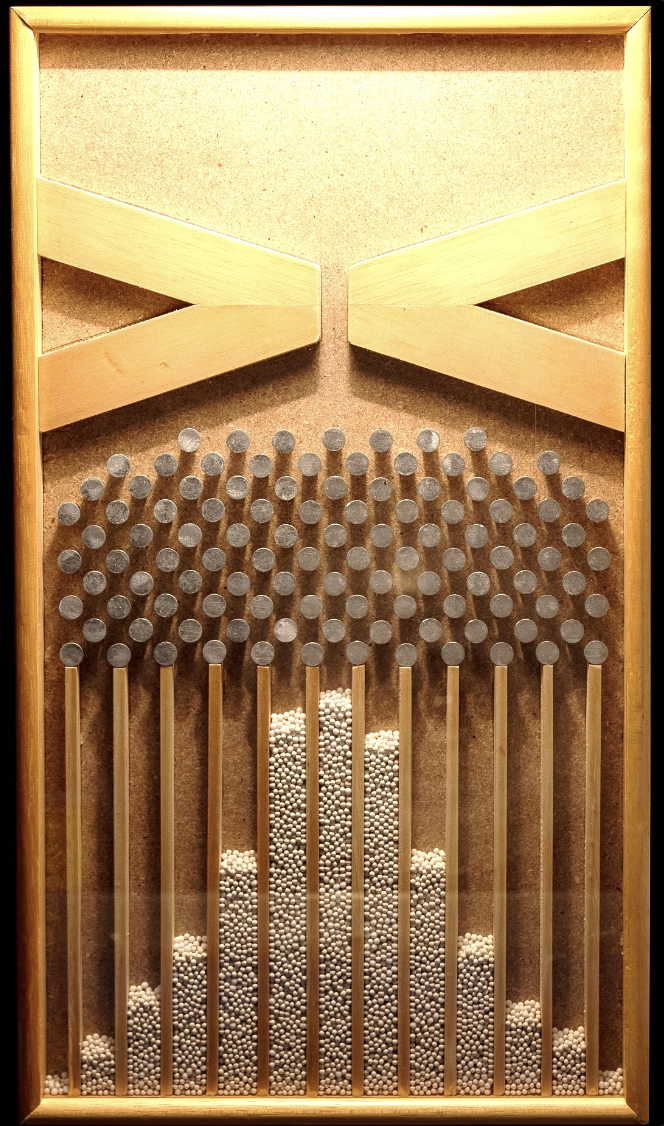
\includegraphics[width=\textwidth]{assets/images/q2d1.png}
            \caption{A Galton board with $h = 10$ (ignore the leftmost and
            rightmost pockets).}
            \label{fig_q2d1}
        \end{subfigure}
        \begin{subfigure}[r]{0.4\textwidth}
            \centering
            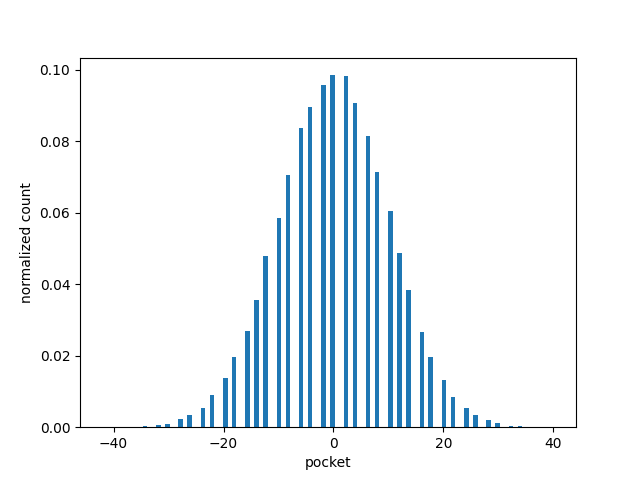
\includegraphics[width=\textwidth]{assets/images/q2d2.png}
            \caption{A simulation with $N = 10^5$ and $h = 100$.}
            \label{fig_q2d2}
        \end{subfigure}
        \caption{Question 2, Task D}
        \label{fig_q2d}
    \end{figure}
    
    Consider simulating the motion of a large number $N$ of balls along the Galton
    board, and record the fraction of balls that finally end up in each of the $h 
    + 1$ pockets.

    The simulation works by simulating the motion of each ball from the top to the
    bottom of the Galton board. Initially, the ball is at $x = 0$. In the first
    step, the ball moves left or right with equal probability - so its current
    position $x$ is incremented or decremented with equal probability. The second
    step is identical - with a different starting position $x$. Suppose in the
    first step $x$ was incremented, so $x = 1$ now. Then, in the second step, $x$
    is decremented (back to 0) or incremented (to 2) with equal probability.
    Perhaps it was incremented again. The third step decrements it to 1 or
    increments it to 3 with equal probability. Maybe it was decremented to 1. A
    fourth step takes it to 0 or 2 with equal probability. And so on. $h$ steps
    ensue till the final value of its position $x$ is the pocket the ball will
    fall into.
    
    The choice of moving left or right can be simulated by simulating from \{0, 
    1\} uniformly randomly (find a function in \texttt{numpy.random} to do this). 
    $h$ uniform samples from \{0, 1\} thus allow us to simulate one ball.

    The process can be repeated $N$ times, with the final pockets of each
    simulated ball being recorded to yield a simulation of the Galton board.

    Your task is to carry out this simulation for $N = 1000$ for the three values
    $h = 10, 50, 100$ of the depth of the board. For each value of $h$, plot the
    counts of balls in each pocket obtained as a histogram, with one bin for each
    pocket. The code is to be written in file \texttt{2d.py}, with the three
    histograms saved to files \texttt{2d1.png}, \texttt{2d2.png} and
    \texttt{2d3.png} (see figure \ref{fig_q2d2} for a reference plot). What do you
    notice about the shape of the tops of the histogram?  
\end{tcolorbox}

% Solution D

\vspace{10pt}
\noindent To simulate the Galton board, we can write a code as in
code:\ref{code:2.2}.

\begin{lstlisting}[
caption={The code to stimulate a Galton board},
label={code:2.2}
]
import numpy as np


def simulate_galton_board(depth: int, number_of_balls: int) -> np.ndarray:
    """
    Simulates the Galton board with depth h and N balls.
    """
    
    # Random movement sequence, less than 0.5 = left, greater than 0.5 = right.
    random_movement = np.random.uniform(0, 1, (number_of_balls, depth))
    movement_array = np.where(random_movement < 0.5, -1, 1)
    
    final_positions_galton_board = np.sum(movement_array, axis=1)
    return final_positions_galton_board
\end{lstlisting}

Here, we generate a random sequence of L and R for every ball, and calculate the final position for all the balls and output this array.

The simulations for N = 1000 and h = \{10, 50, 100\} give the images \ref{fig_a2d1}, \ref{fig_a2d2} and \ref{fig_a2d3}:

\begin{figure}[H]
    \centering
    \begin{subfigure}{0.4\textwidth}
        \centering
        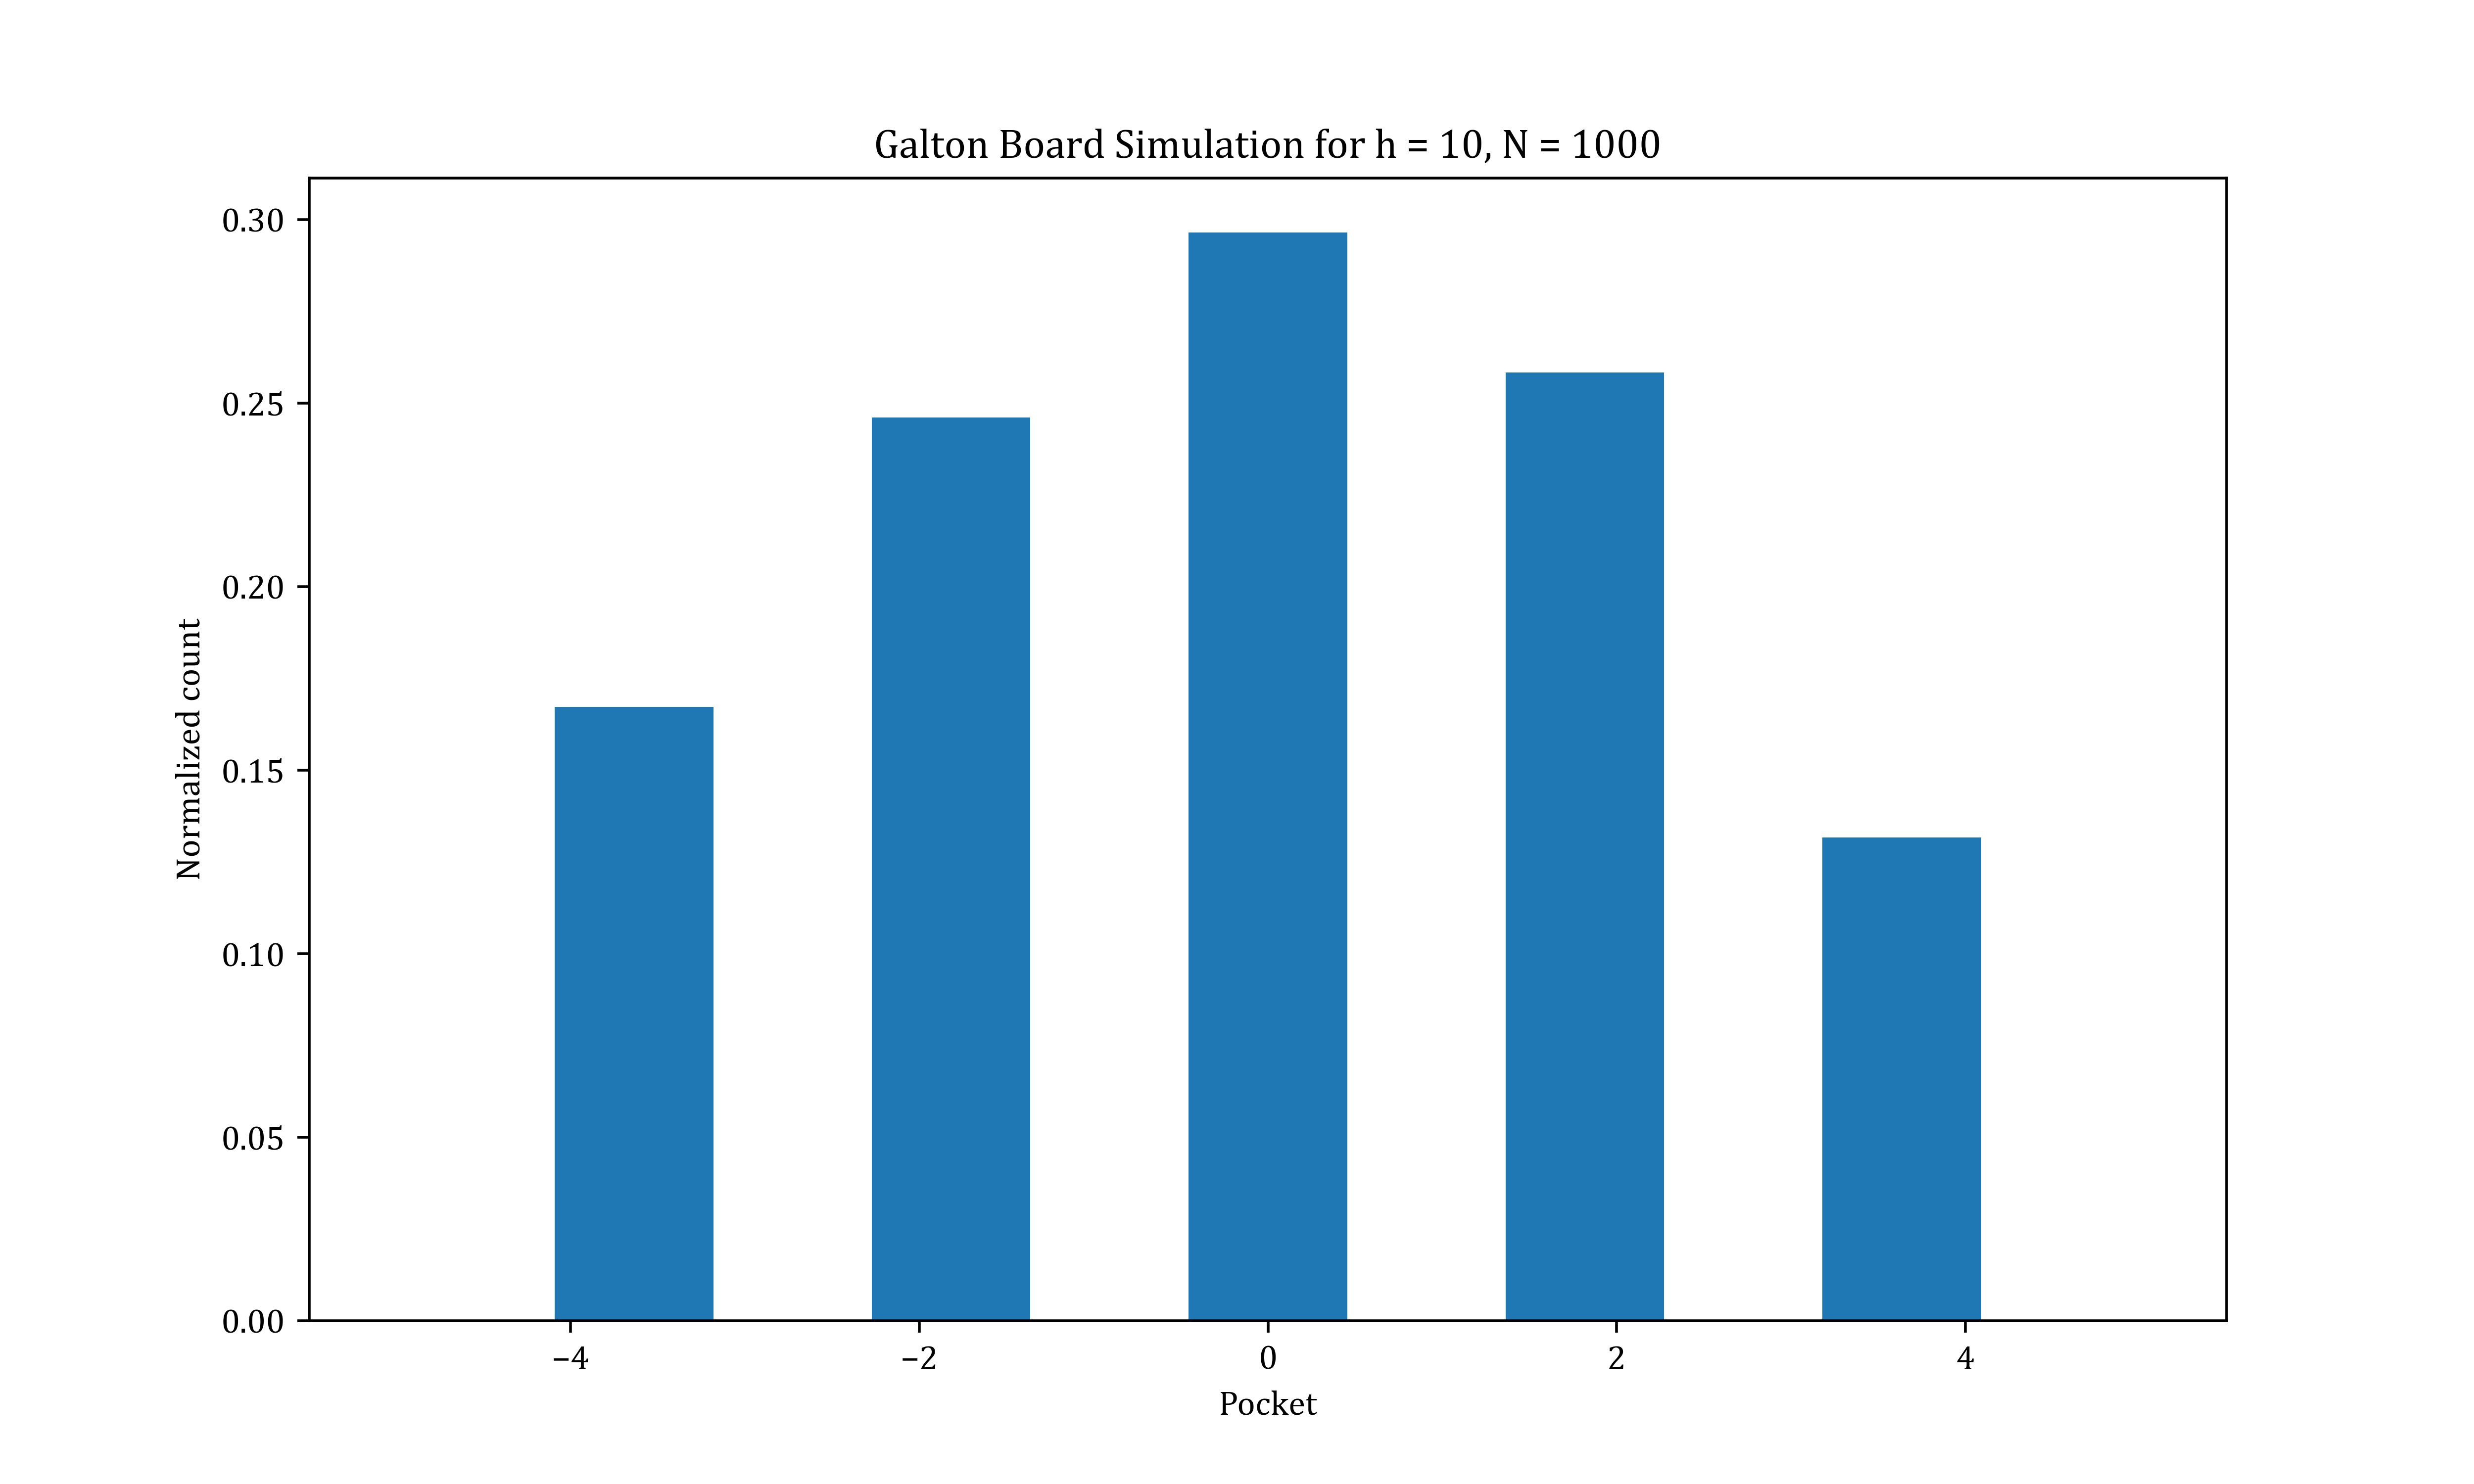
\includegraphics[width=\textwidth]{assets/images/a2d1.png}
        \caption{$N = 1000, h = 10$}
        \label{fig_a2d1}
    \end{subfigure}
    \begin{subfigure}{0.4\textwidth}
        \centering
        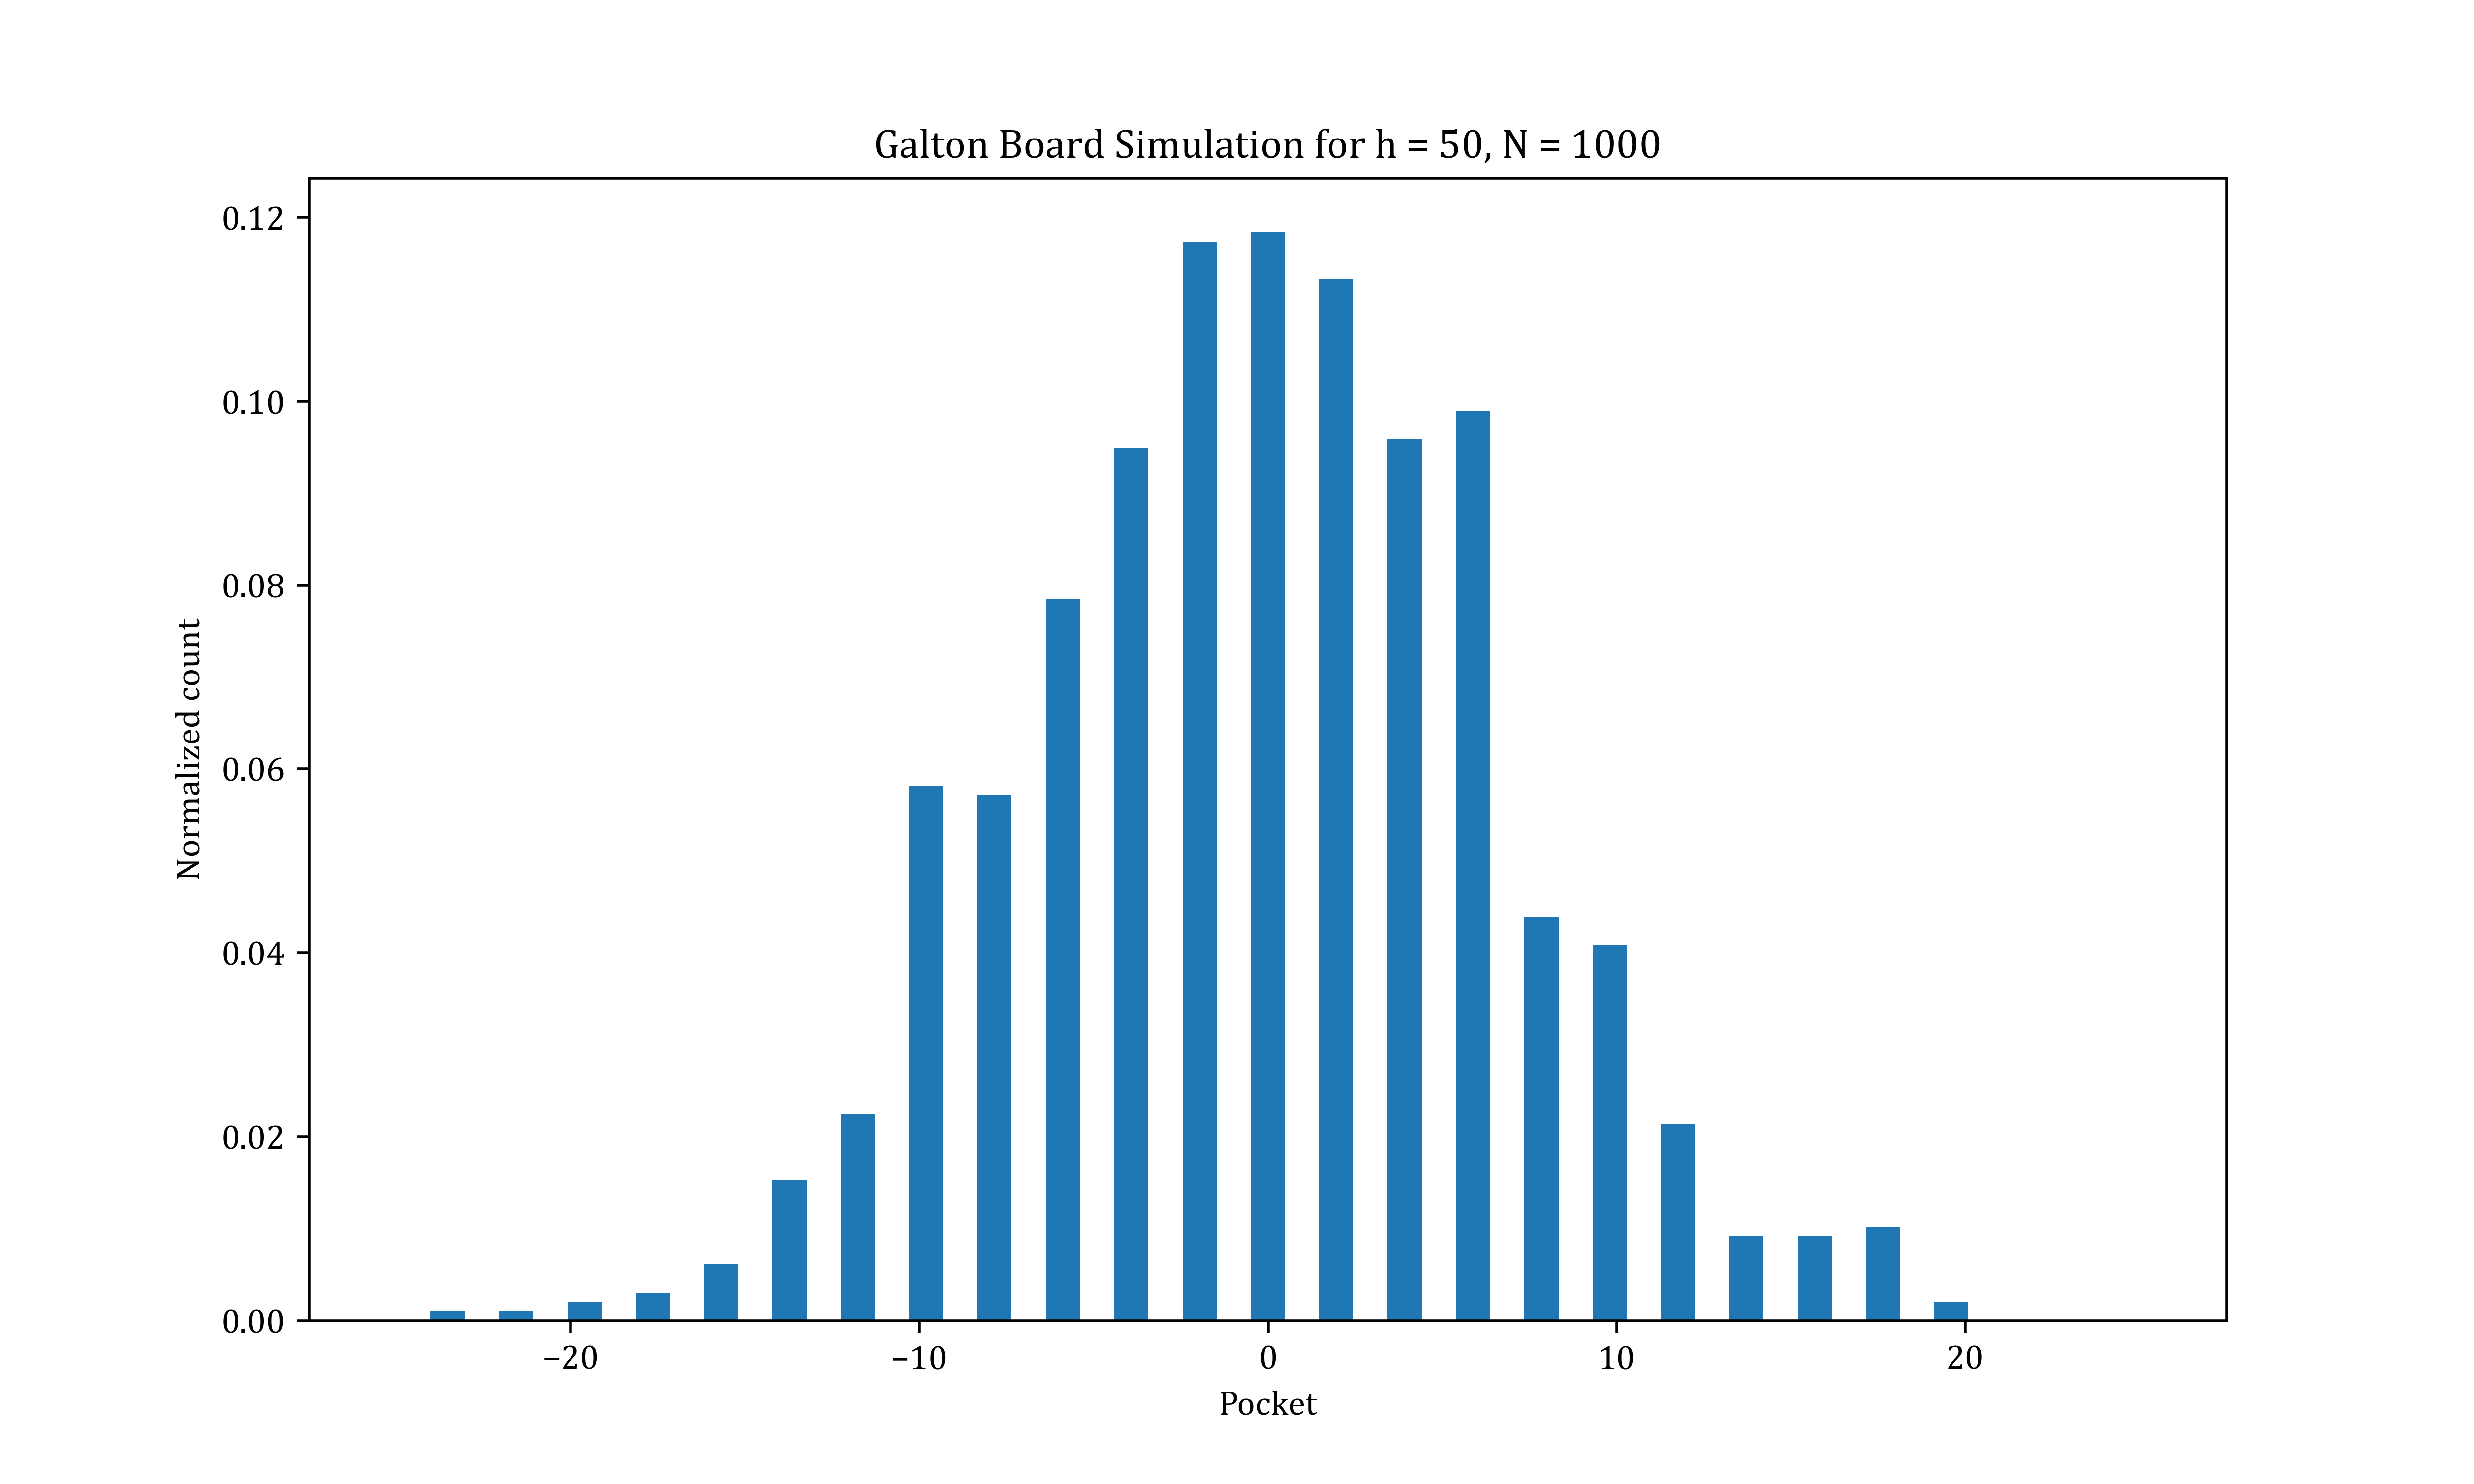
\includegraphics[width=\textwidth]{assets/images/a2d2.png}
        \caption{$N = 1000, h = 50$}
        \label{fig_a2d2}
    \end{subfigure}
    \begin{subfigure}{0.4\textwidth}
        \centering
        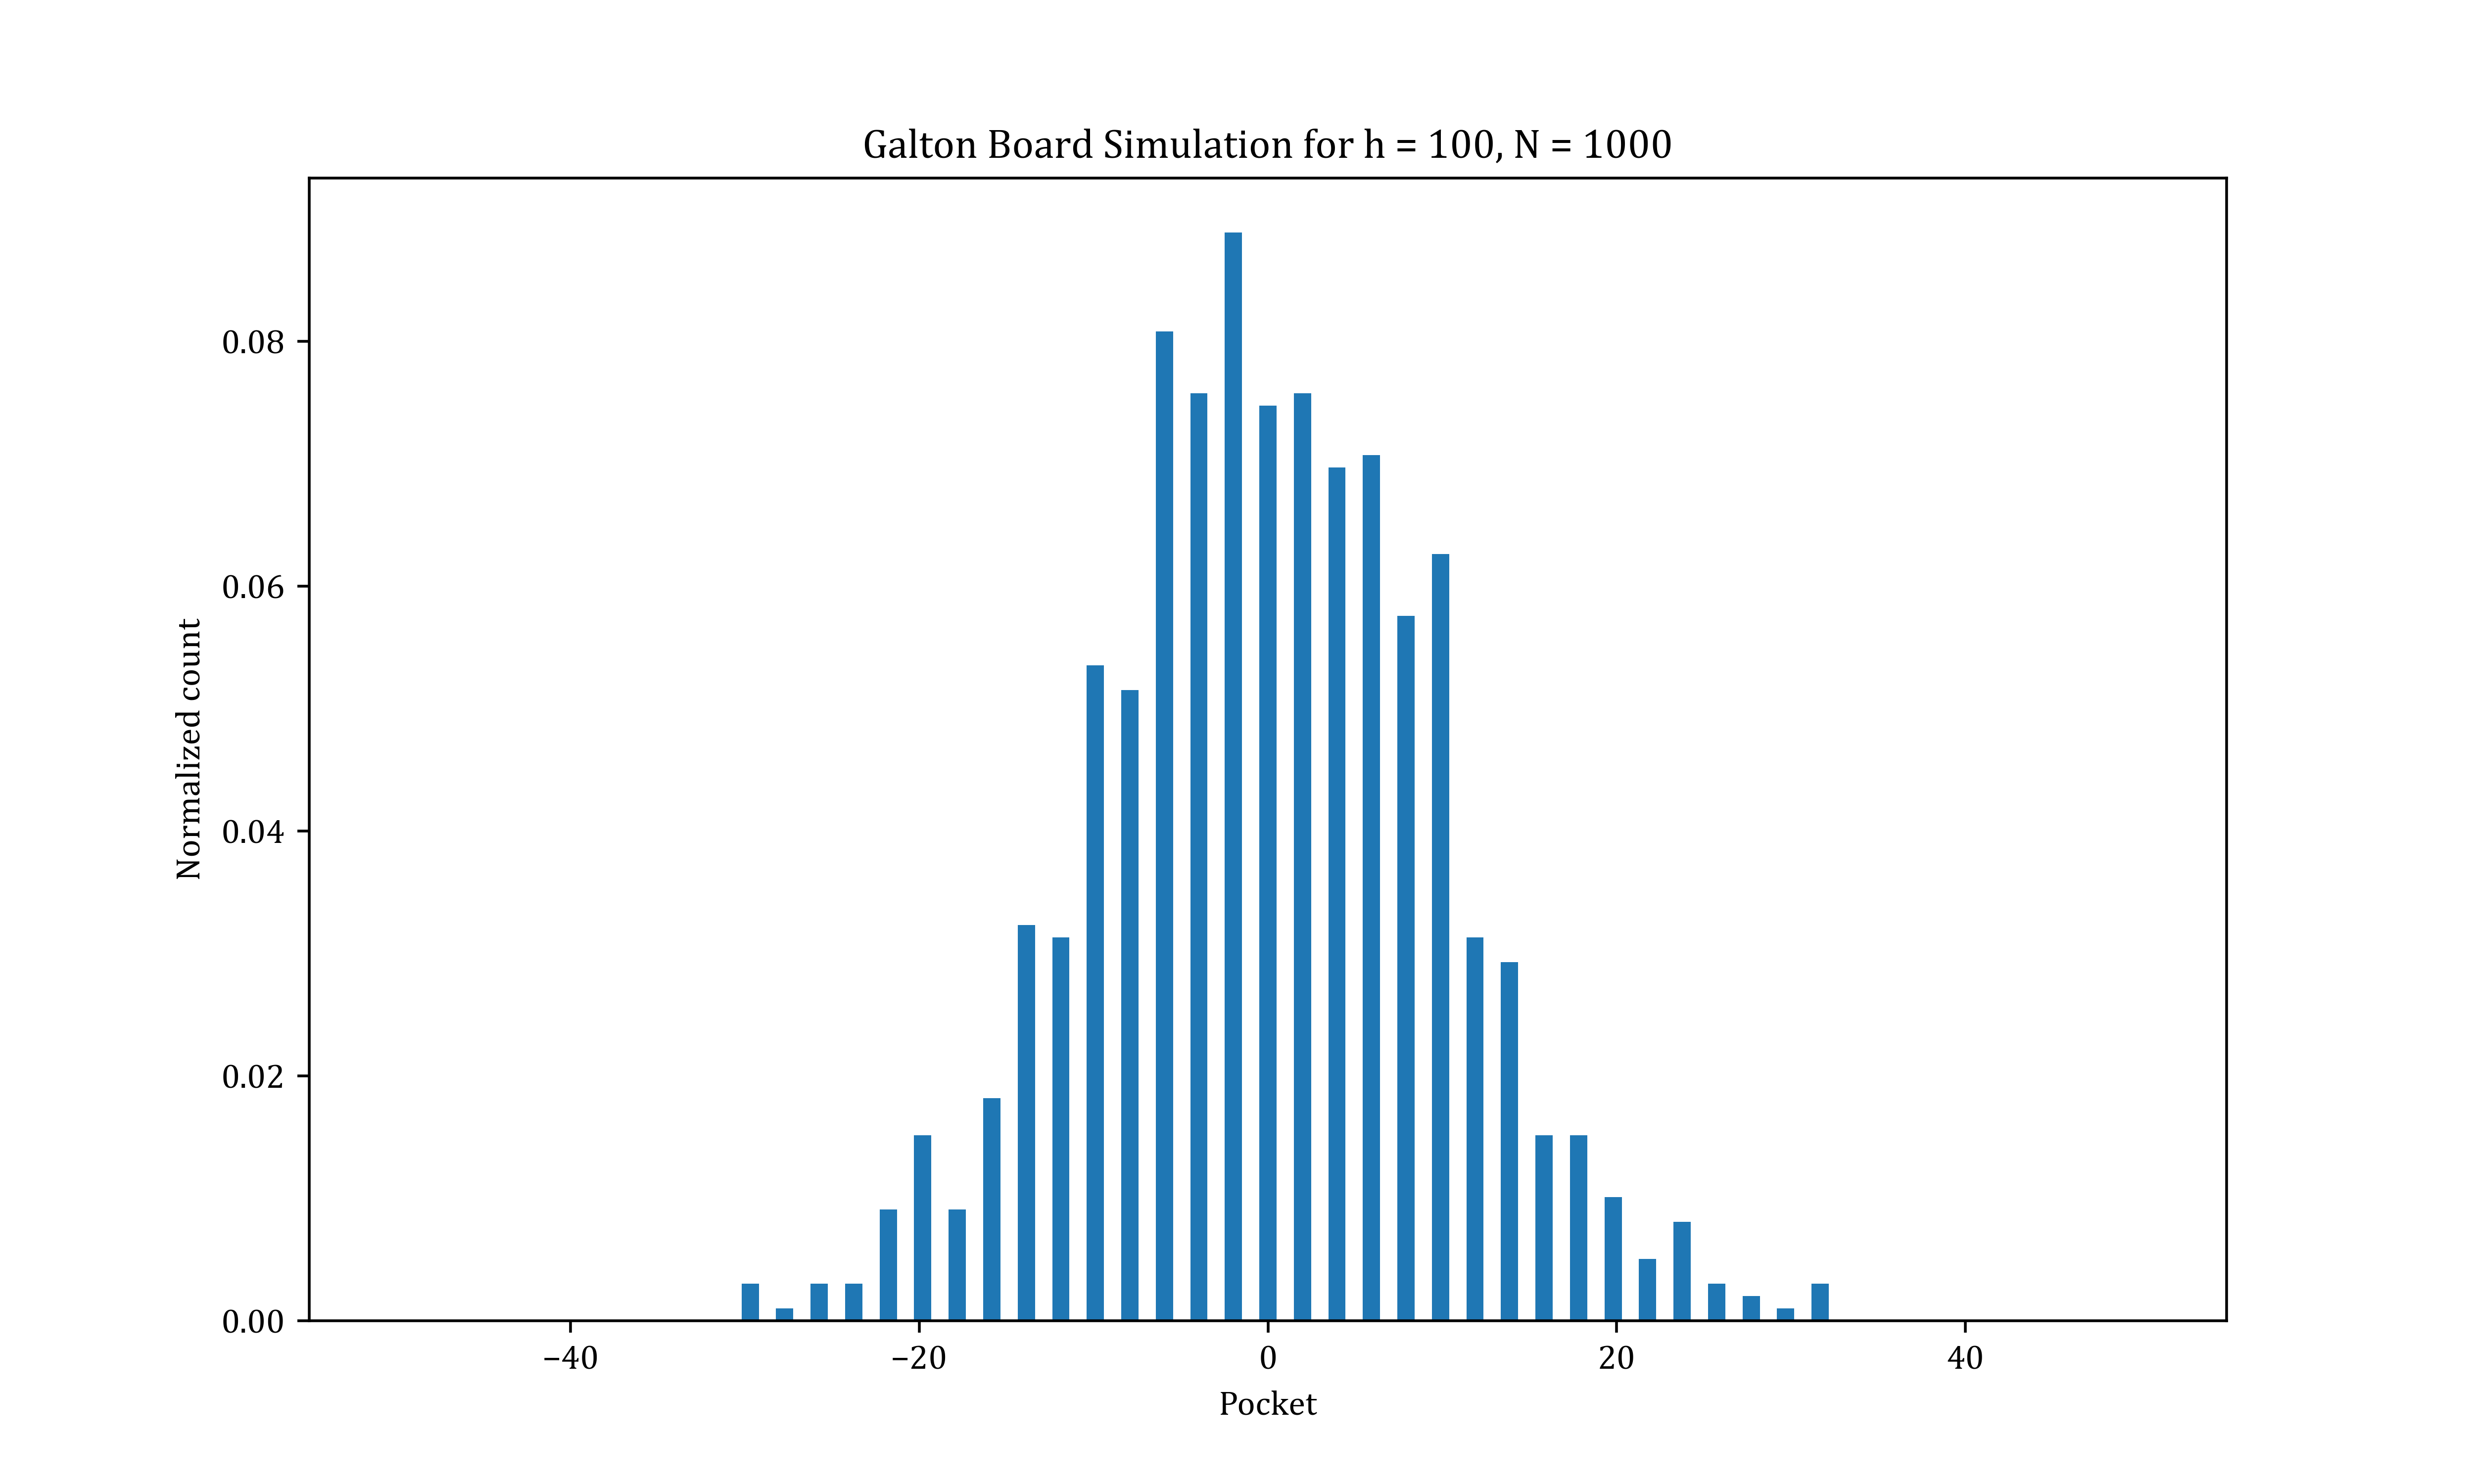
\includegraphics[width=\textwidth]{assets/images/a2d3.png}
        \caption{$N = 1000, h = 100$}
        \label{fig_a2d3}
    \end{subfigure}
    \begin{subfigure}{0.4\textwidth}
        \centering
        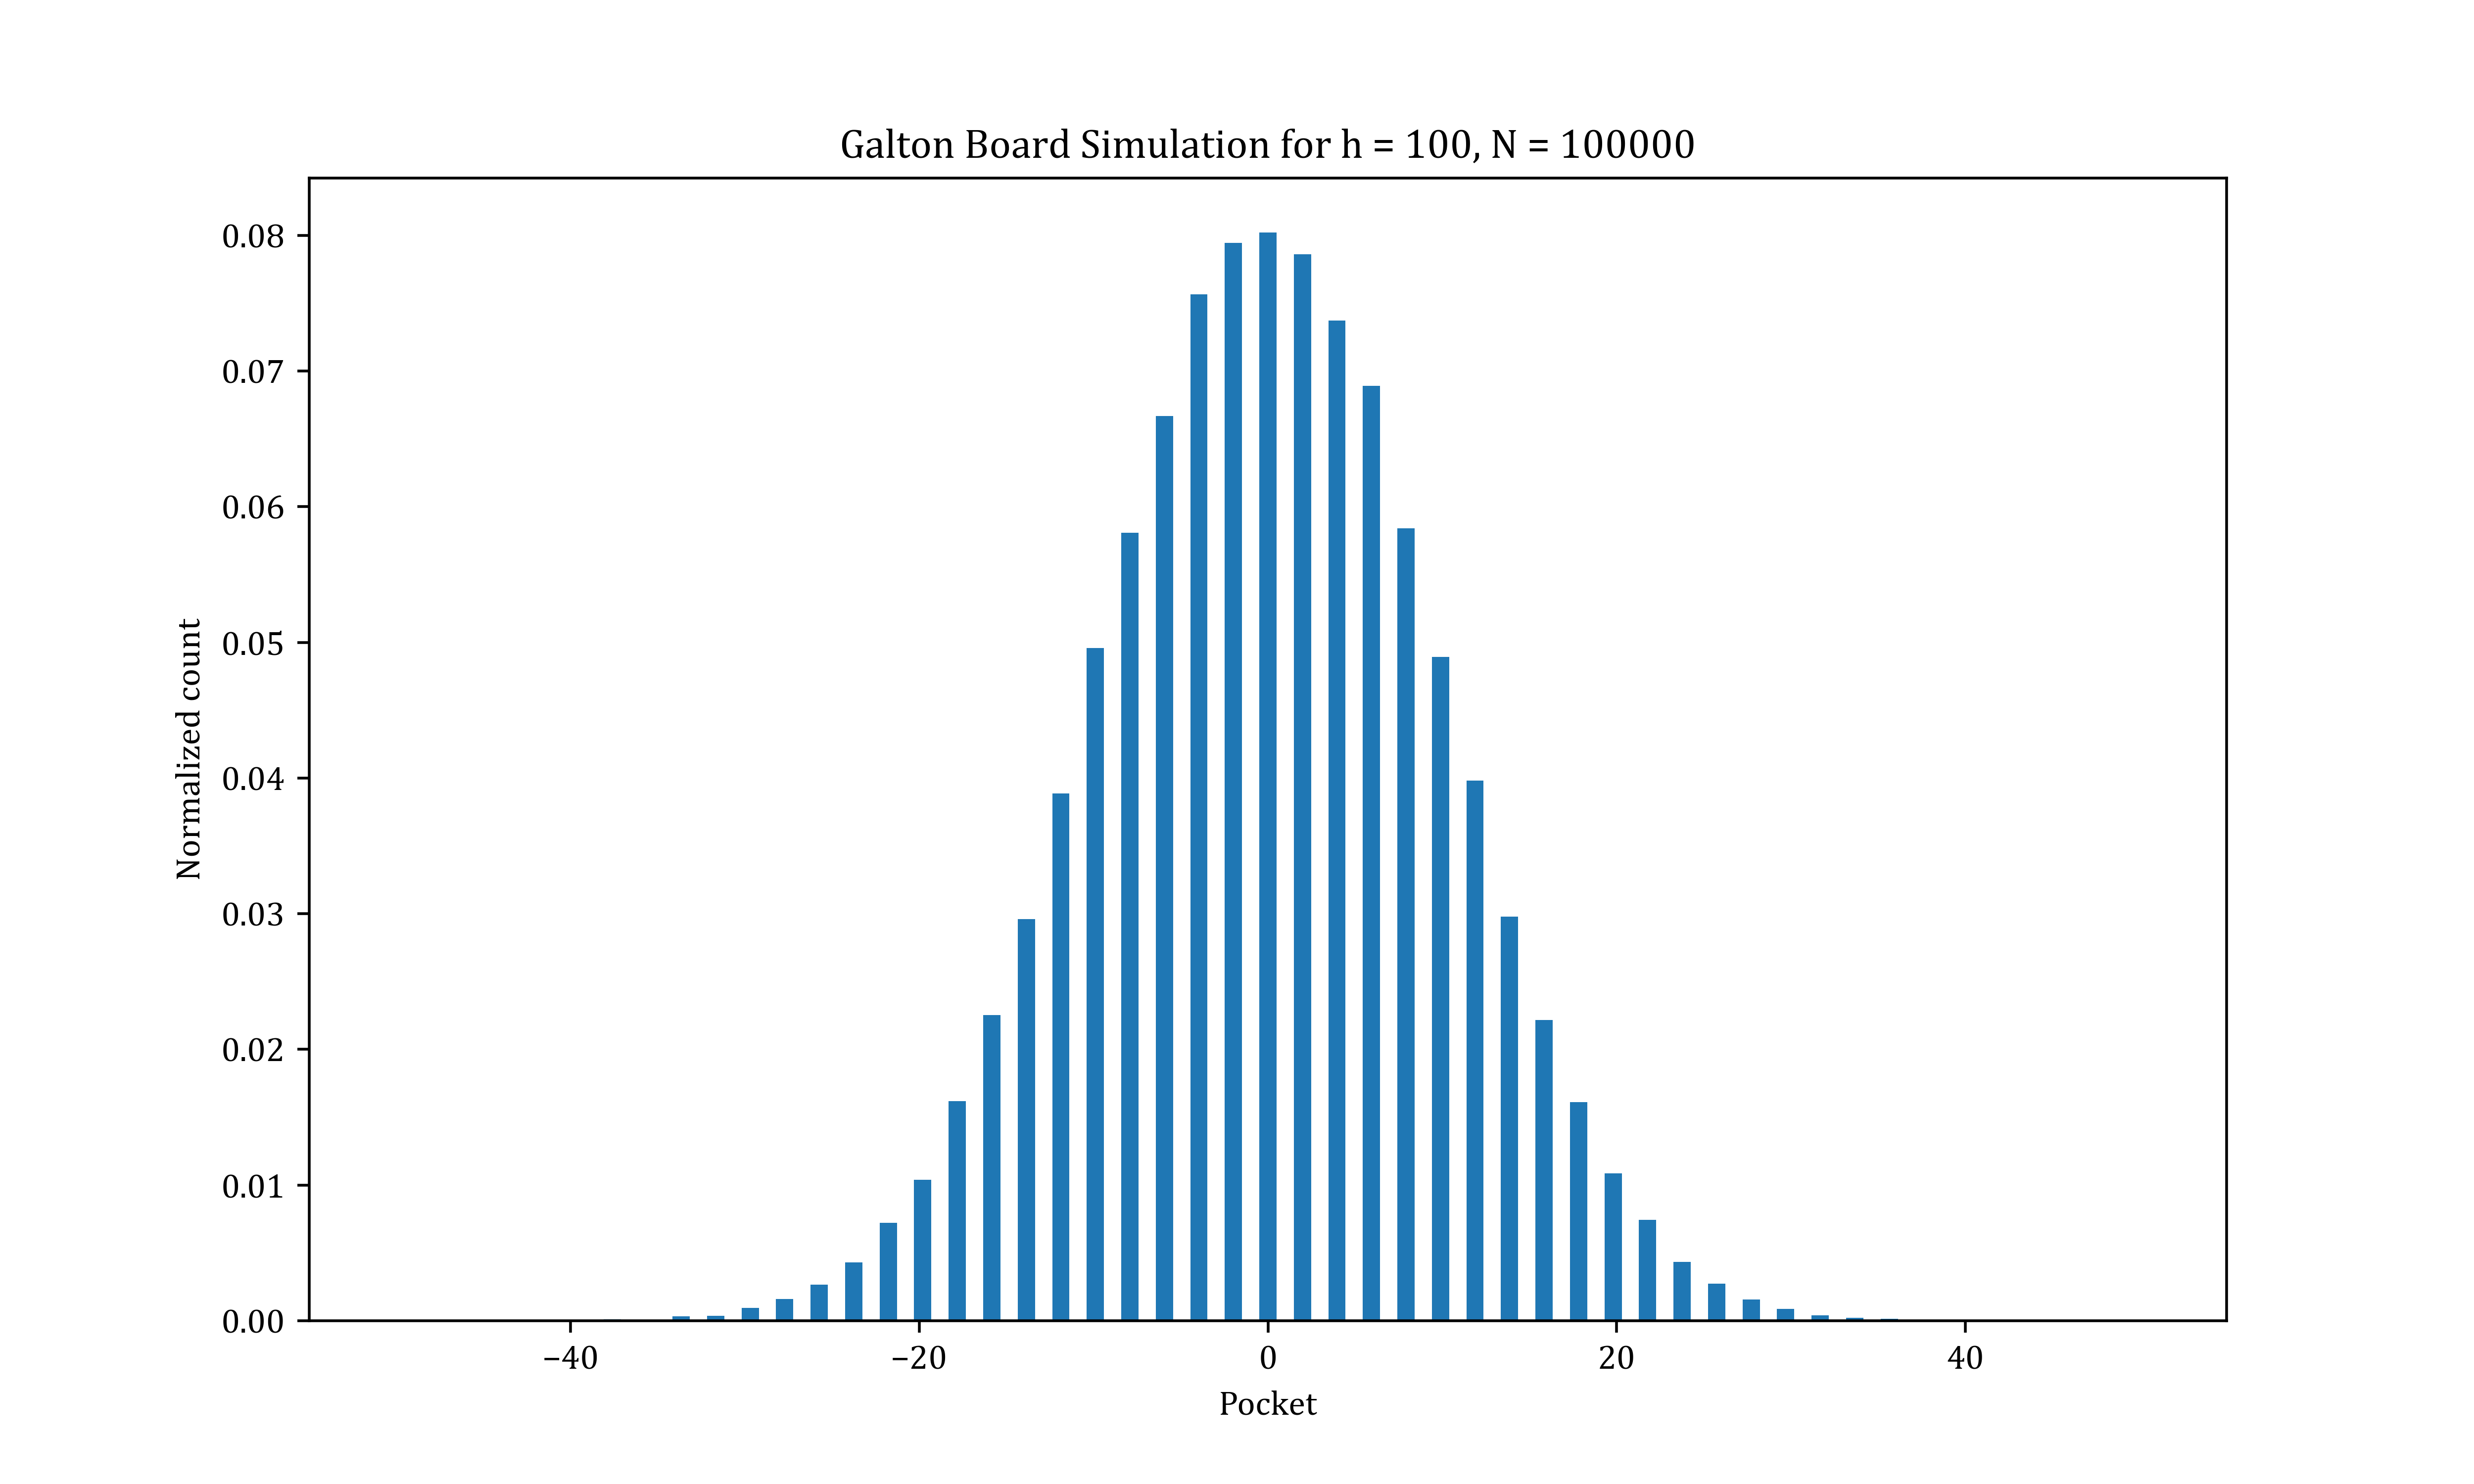
\includegraphics[width=\textwidth]{assets/images/a2d4.png}
        \caption{$N = 10^5, h = 100$}
        \label{fig_a2d4}
    \end{subfigure}
    \caption{Simulations for various $h$ (Depth) and $N$ (Dumber of balls)}
\end{figure}

\subsection*{Code and Image locations}

To generate the images, no special instructions required, just running the code
\texttt{code/2d.py} will generate the images.

\vspace{10pt}
\noindent The files:
\begin{itemize}
    \item[$\bullet$] \texttt{code/2d.py}
    \item[$\bullet$] \texttt{images/2d1.png}
    \item[$\bullet$] \texttt{images/2d2.png}
    \item[$\bullet$] \texttt{images/2d3.png}
\end{itemize}

\section*{\colS{$\S$} Task E (B) \hfill \normalfont \large [5]}

\begin{tcolorbox}
    The goal is to theoretically show that the number of balls in each pocket is
    normally distributed. Suppose that $h = 2k$ is even. Consider a Galton board
    of depth $h$. Let random variable $X \in \{-h, -h + 2, \ldots, 0, 2, \ldots,
    h - 2, h\}$ describe the pocket in which a ball finally lands (notice that
    $X$ can only be even). The probability mass distribution $P_h[\cdot]$ of $X$
    is determined by the randomness of the outcome of each collision. There are
    two sub-tasks here.
    
    \vspace{10pt}
    \begin{itemize}
        \item Compute (in closed form)the value $P_h[X = 2i]$ for each $i \in \{-
        k, -k + 1, \ldots, k - 1, k\}$.
        \item Show that for large enough $h$ and even $i \ll \sqrt{h}$,
        
            \begin{equation*}
                P_h[X = i] \approx \dfrac{1}{\sqrt{\pi k}}e^{-\frac{i^2}{k}}
                = \mathcal{N}\left(\mu = 0, \sigma^2 = \dfrac{k}{2}\right)(i).
            \end{equation*}

        You may need to use Stirling’s approximation for the factorial.

            \begin{equation*}
                n! \approx \sqrt{2\pi n}\left(\dfrac{n}{e}\right)^n
            \end{equation*}

        to solve this sub-task.
    \end{itemize}
\end{tcolorbox}

% Solution E

\subsection*{The PMF in closed format}

As $X = 2i$ can be achieved by arranging a particular number of Ls and Rs (which
can be calculated) in a random order and as the sample space is the total number
of ways to get a string of Ls and Rs (From the way how a Galton board's
distribution is generated in the code \ref{code:2.2}).

Now, to calculate the numbers of Ls and Rs: The sum of all the Ls(1) and Rs(-1)
is $2i$, which means out of the $h$ characters, we have $2i$ Ls and the rest are
an equal amount of Ls and Rs.

\begin{equation*}
    \begin{aligned}
        \text{Number of Ls} &= 2i + \dfrac{h - 2i}{2} = \dfrac{h}{2} + i \\
        \text{Number of Rs} &= \dfrac{h - 2i}{2} = \dfrac{h}{2} - i
    \end{aligned}
\end{equation*}

$P_h[X = 2i]$ can be rewritten as:

\begin{equation}
    \begin{aligned}
        P_h[X = 2i] = \dfrac{\text{Number of ways to arrange $\frac{h}{2} + i$ Ls
        and $\frac{h}{2} - i$ Rs}}{\text{The total number of ways to get a string
        of Ls and Rs}}
    \end{aligned}
    \label{e2.6}
\end{equation}

Using the principles of counting on \ref{e2.6}:

\begin{equation}
    \begin{aligned}
        P_h[X = 2i] =
        \dfrac{h!}{
        \left(\dfrac{h}{2} + i\right)! \cdot
        \left(\dfrac{h}{2} - i\right)! \cdot
        2^h}
    \end{aligned}
    \label{e2.7}
\end{equation}

Equation \ref{e2.7} is the closed form of $P_h[X = 2i]$.

\subsection*{Approximation for a large $h$}

I am writing the expression for $P_h[X = 2i]$ as $P_h[X = i]$ when $i$ is odd
doesn't make sense.

\vspace{10pt}
\noindent For large $h$, we use the Stirling's approximation on the factorials
from the equation \ref{e2.7} to get

\begin{equation}
    \begin{aligned}
        P_h[X = 2i] \approx
        \dfrac{\sqrt{2\pi h}\left(\dfrac{h}{e}\right)^h}
        {\sqrt{2\pi \left(\dfrac{h + 2i}{2}\right)}
        \left(\dfrac{h + 2i}{2e}\right)^{\dfrac{h + 2i}{2}} \cdot
        \sqrt{2\pi \left(\dfrac{h - 2i}{2}\right)}
        \left(\dfrac{h - 2i}{2e}\right)^{\dfrac{h - 2i}{2}} \cdot
        2^h}
    \end{aligned}
    \label{e2.8}
\end{equation}
Simplifying (rearranging powers, cancelling terms, no approximations) \ref{e2.8}
gives

\begin{equation}
    \begin{aligned}
        P_h[X = 2i] \approx
        \dfrac{\sqrt{2}}
        {\sqrt{\pi h}\left(1-\dfrac{4i^{2}}{h^{2}}\right)^{\dfrac{h + 1}{2}} \cdot
        \left(\dfrac{h + 2i}{h - 2i}\right)^i}
    \end{aligned}
    \label{e2.9}
\end{equation}

\subsubsection*{Now approximating:}

We begin by simplifying the term:

\begin{equation*}
    \left( 1 - \dfrac{4i^2}{h^2} \right)^{\dfrac{h + 1}{2}}
\end{equation*}
For large $h$, we assume that $\dfrac{i^2}{h^2}$ is small. We can then
use the binomial expansion (or a Taylor series expansion) for small $x$, which
states:

\begin{equation*}
    (1 - x)^n \approx e^{-nx} \text{ for small } x
\end{equation*}
Here, $x = \dfrac{4i^2}{h^2}$ and $n = \dfrac{h + 1}{2}$, so we
approximate:

\begin{equation*}
    \left( 1 - \dfrac{4i^2}{h^2} \right)^{\dfrac{h + 1}{2}} \approx
    \exp {\left(-\dfrac{h + 1}{2} \cdot \dfrac{4i^2}{h^2}\right)}
\end{equation*}
For large $h$, the factor $\dfrac{h + 1}{2}$ is approximately
$\dfrac{h}{2}$, so this simplifies further to:

\begin{equation*}
    \exp{\left(-\frac{h}{2} \cdot \frac{4i^2}{h^2}\right)} =
    e^{-\frac{2i^2}{h}}
\end{equation*}

\begin{equation}
    \implies \left( 1 - \dfrac{4i^2}{h^2} \right)^{\dfrac{h+1}{2}} \approx
    e^{-\frac{2i^2}{h}}
    \label{e2.10}
\end{equation}

\vspace{20pt}
\noindent Next, we simplify the term:

\begin{equation*}
    \left(\dfrac{h + 2i}{h - 2i}\right)^i
\end{equation*}
For large $h$, we can use the logarithmic approximation. First, express
the ratio as:

\begin{equation*}
    \dfrac{h + 2i}{h - 2i} = 1 + \dfrac{4i}{h - 2i}
\end{equation*}
For large $h$, $h - 2i \approx h$, so we approximate the ratio as:

\begin{equation*}
    \dfrac{h + 2i}{h - 2i} \approx 1 + \dfrac{4i}{h}
\end{equation*}
Now, we apply the logarithmic expansion for small $x$, which states:

\begin{equation*}
    \log(1 + x) \approx x \text{ for small } x
\end{equation*}
Thus:

\begin{equation*}
    \begin{aligned}
        \log\left(\dfrac{h + 2i}{h - 2i}\right) &\approx \dfrac{4i}{h} \\
        \left(\dfrac{h + 2i}{h - 2i}\right)^i &\approx
        \exp{\left(i \cdot \dfrac{4i}{h}\right)}
        = e^{\frac{4i^2}{h}}
    \end{aligned}
\end{equation*}

\begin{equation}
    \implies \left(\dfrac{h + 2i}{h - 2i}\right)^i \approx e^{\frac{4i^2}{h}}
    \label{e2.11}
\end{equation}
Using \ref{e2.10} and \ref{e2.11} in \ref{e2.9}, we get

\begin{equation}
    \begin{aligned}
        P_h[X = 2i] &\approx
        \dfrac{\sqrt{2}}{\sqrt{\pi h}} \cdot
        \dfrac{1}{e^{-\frac{2i^2}{h}} \cdot
        e^{\frac{4i^2}{h}}} \\
        \implies P_h[X = 2i] &\approx
        \dfrac{1}{\sqrt{\pi \left(\dfrac{h}{2}\right)}} \cdot
        e^{\frac{-i^2}{\left(\frac{h}{2}\right)}} \\
        \implies P_h[X = 2i] &\approx
        \dfrac{1}{\sqrt{\pi k}} \cdot
        e^{\frac{-i^2}{k}}
    \end{aligned}
    \label{e2.12}
\end{equation}
Comparing this result from \ref{e2.12} with the Gaussian form

\begin{equation*}
        \dfrac{1}{\sqrt{2 \pi \sigma^2}} \cdot e^{\frac{-i^2}{2 \sigma^2}},
\end{equation*}
We get $2\sigma^2 = k$.

\vspace{10pt}
\noindent So, $P_h[X = 2i]$ is a Gaussian in $i$, with its variance
$\sigma^2 = \dfrac{k}{2}$, as represented in \ref{e2.13}.

\begin{equation}
    \begin{aligned}
        P_h[X = 2i] &\approx
        \mathcal{N}\left(\mu = 0, \sigma^2 = \dfrac{k}{2}\right)(i) \\
        &\text{(or)} \\
        P_h[X = 2i] &\approx
        \mathcal{N}\left(\mu = 0, \sigma^2 = \dfrac{h}{4}\right)(i) \\
        \text{for } &i \ll \sqrt{h}.
    \end{aligned}
    \label{e2.13}
\end{equation}
